% -*- root: ../paper.tex -*-

Matcher functions in \systemname come from three places: Learned Heuristics, Expert Augmentations, and User Feedback. 
In this Section, we address the first of these three.
Because the learned heuristics are only the first step in an iterative process, our goal is not to develop an exhaustively correct matching scheme.
Rather, we want something that is both simple and fast.
Accordingly, throughout this section we make several simplifying assumptions.




\subsection{Learning Matchers}
Specific modeling techniques vary by data type, so our first step was to assess what types exist.
We sampled a collection of 62 data sets from open data portals. 
%, as discussed later in Experiments (Section~\ref{sec:experiments}).

We then categorized the 458 columns in our sample into three broad types: 
(1) Numeric data, or any records consisting of digits, at most a single decimal point, and an optional exponent; 
(2) Enumerated types, based on an arbitrary threshold of atleast 50\% distinct values in the column; and 
(3) Textual data, or anything else.  
By far, the dominant type was numeric, so the preliminary efforts we outline in this paper focus on modeling exclusively \emph{numeric} data.

Regardless of the specific data type however, the overall learning process is similar.

The input to the process is a collection of labeled tabular data.  
Each column is split out and a type-specific modeling process is run for each column's data pair.
The output of the modeling process is zero or more matchers that reliably model the column.
If the process returns at least one matcher, we instantiate a new concept node with the column's name.
We then add nodes for each matcher returned by the modeling process and edges to the newly instantiated concept node.

\subsection{Creating Matchers for Numeric Data}
We considered a range of options for modeling numeric data and settled on an approach based on numerical distributions.
In comparison to more complex approaches like neural networks, this approach is simple, efficient, and well understood.
Simply put, given a number of example column instances, we explore a range of numerical distributions and select the one with the best fit.
Our preliminary implementation of \systemname explores three different distributions: Uniform, Normal, and Log-normal. 

\begin{figure}
	\centering
	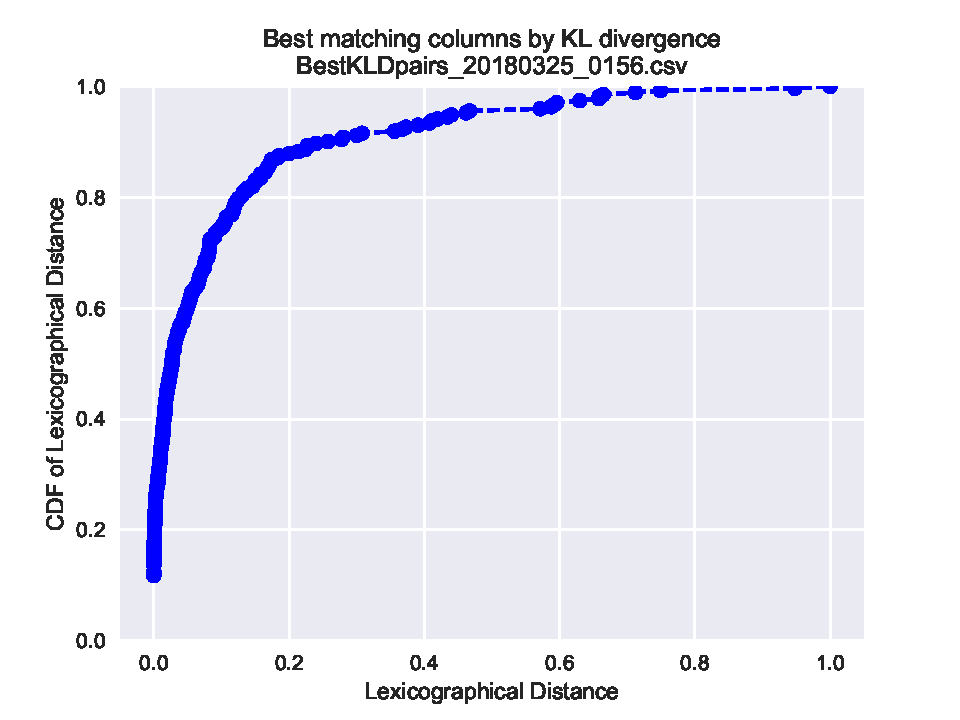
\includegraphics[trim={0 6mm 0 0},clip,width=1\columnwidth]{graphics/CDF_LexDistance1}
	\caption{CDF of Lexicographical Distance for the best match for each column.}
	\label{fig:cdflexdist}
	\trimfigurespacing
\end{figure}

We used Kullback-Leibler (KL) divergence to measure how one distribution diverges from from another. A KL divergence of 0 suggess that distributions could be similar, if not the same. A KL divergence of 1 suggests that two distributions are very different. If knowledge of a specific problem domain suggests that similarity of data distributions could be better represented by another measure, KL divergence can be easily swapped with for it in our system.  

Lexicographical Distance indicates the difference in the column labels of two distributions. We used two measures of Lexicographical Distance - Levenstein Distance and NGram Distance. Section~\ref{sec:expertui} talks about performance of both of the measures in estimating Lexicographical Distance on our dataset. A Lexicographical Distance value of 0 suggest that the two columns labels are exactly the same, whereas, a value of 1 suggests that the column labels are very different.

Learned heuristics require an assumption to build baseline match-quality functions. We proceed with the initial assumption that column pairs with \textit{similar} data would be labelled \textit{similarly}. The value of KL divergence of two columns is inversely proportional to \textit{similarity} of their data distributions. The value of Lexicographical distance of two columns is inversely proportional to \textit{similarity} of their column labels. We have verified this assumption by plotting the Cummulative Distribution Function of Lexicographical Distance of column pairs with minimum KL Divergence in Figure~\ref{fig:cdflexdist}. 80\% of column pairs with most similar data have their labels which are at most 0.129 lexical distance apart. This indicates that even without human intervention, columns pairs with the most similar data are already labelled similarly. 
 
For each distribution, we find the parameters ($\ell,h,\mu,\sigma,a$) that minimize the root-mean-squared (RMS) error between the theoritical and empirical distributions. 

$$\mathbb U(\ell, h)\;\;\;\;\;\mathbb N(\mu, \sigma)\;\;\;\;\;\mathbb Lognorm(\mu{*},\sigma{*})$$

Parameter estimation is performed by maximizing a log-likelihood function. Log-likelihood estimation is a widely used and robust technique for estimating the likelihood of a statistical distribution and its parameters being representative of the empirical data distribution. We implemented this using the SciPy package in Python. 

We then select the one distribution with the lowest overall RMS error. The resulting match-quality function is the probability of the column values being a representative sample drawn from this distribution.
% We measure this probability by the \placeholder{RMS Error} between the distribution of the sampled values and the distribution modeling the name.